\section{Introduction}
\label{sec:intro}
This document describes the work of team \textit{model\_car} for the LL4 lab course at \textit{Technische Universität München} in summer 2017. \\

The overall goal of the project is to set up a hardware-in-the-loop (HIL) scenario based on Genode with Fiasco.OC. An image of the scenario is shown in figure \ref{fig:hil}. As one can see, the software part of the HIL is a racing game called \textit{SpeedDreams} which sends control commands to a physical model of a car. The concrete commands sent to the model are braking-, steering-, and acceleration requests. The model car performs the requests in hardware and returns sensor values to the simulation. \\

\begin{figure}[h]
    \centering
    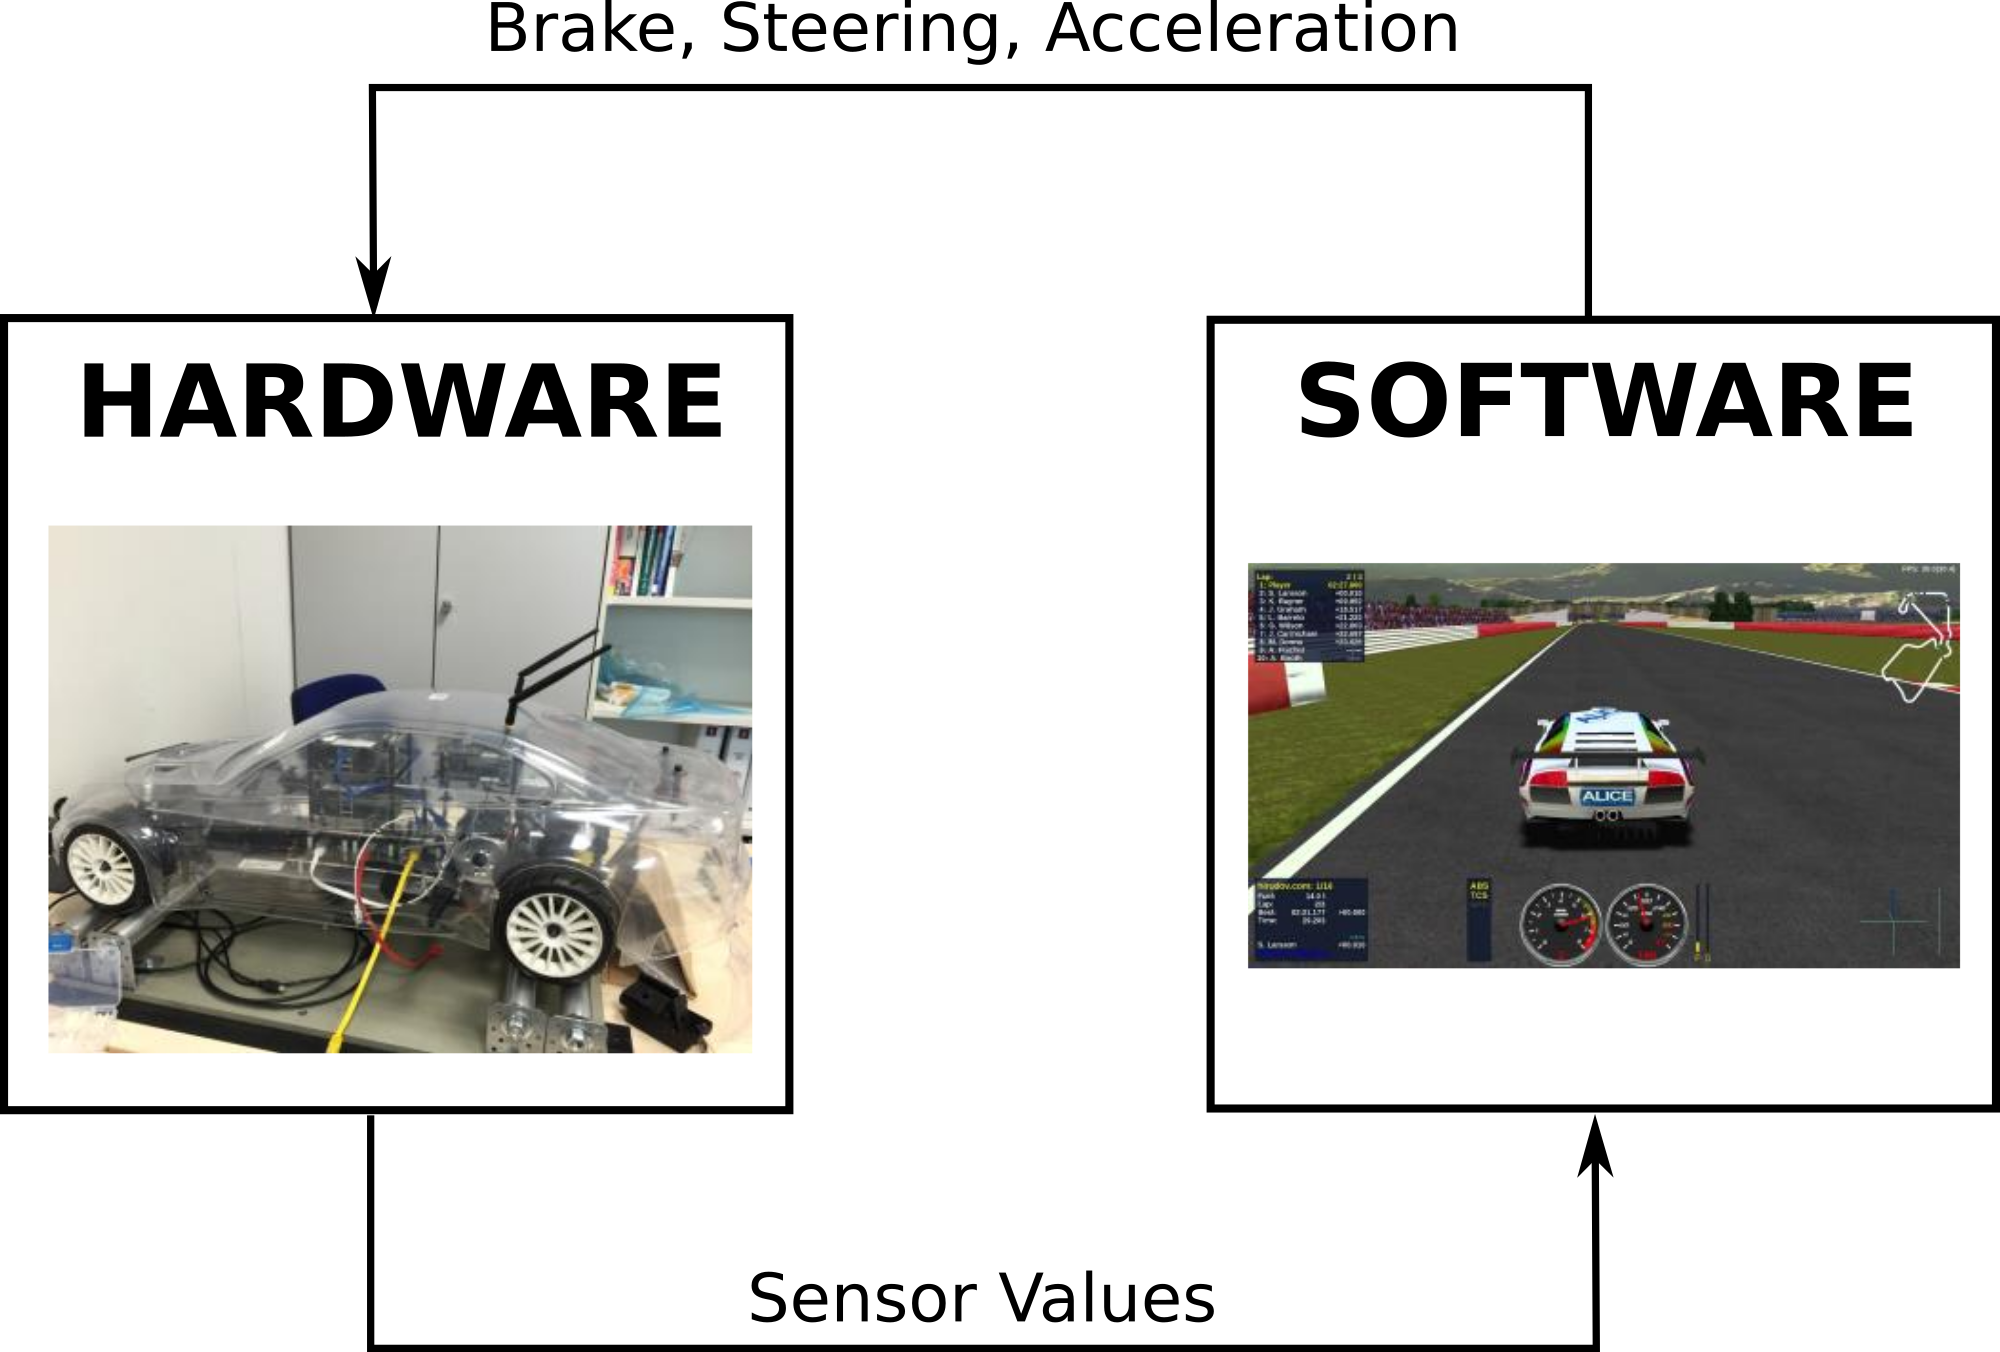
\includegraphics[width=0.7\linewidth]{images/hil}
    \caption{HIL scenario with SpeedDreams and a physical model of a car}
    \label{fig:hil}
\end{figure}

This document describes the hardware part of the HIL, whereas the software part is implemented by another team of the lab course. \\

The project team consists of three master students at the \textit{Technische Universit München}. Florian Mauracher and Christoph Griesbeck study \textit{Computer Science} in the fourth and second semester, respectively. Thomas Mauerer, on the other hand, studies \textit{Automotive Software Engineering} in his third semester.
